\documentclass[letterpaper,spanish,12pt]{report} 
\usepackage[lmargin=2.3cm,
rmargin=2.3cm,top=2.5cm,bottom=2.5cm]{geometry}
\usepackage[spanish]{babel}
\usepackage[utf8]{inputenc}%Con eso pueden directamente escribir acentos en teclados con códificación UTF8
\usepackage{graphicx}
\usepackage{subfigure}
\usepackage{listings}
\begin{document}
%Portada%
\begin{titlepage}
\begin{center}
\vspace*{2cm}
\begin{figure}[htp]
\centering

\includegraphics[scale=0.3]{logo}
\end{figure}
\large{INSTITUTO TECN\'OLOGICO DE MORELIA\\ DEPARTAMENTO DE INGENIER\'IA ELECTR\'ONICA}
\rule{150mm}{0.1mm}\vspace{1.2cm} 
{\bf\Large CONTROL I}\\\vspace{0.8cm} {\bf{\huge Practica No. 1}\\ {\LARGE SISTEMAS DE PRIMER ORDEN}}\\\vspace{0.8cm} 
\begin{tabular*}{15cm}{l@{\extracolsep{\fill}}l}
{\Large Ariadne Paola Gonz\'alez Gallegos} & {\Large 13121114}\\
{\Large Jos\'e Abel Guti\'errez \'Alvarez} & {\Large 13121117}\\
\end{tabular*}
\vspace{0.8cm}\\\rule{150mm}{0.1mm}
\end{center}
\end{titlepage}
\tableofcontents \cleardoublepage
\addcontentsline{toc}{chapter}{Introducci\'on}
%Fin de la portada inicio del reporte%
\chapter*{Introducci\'on}
Para poder analizar un sistema de control es necesario obtener un modelo matem\'atico que describa el funcionamiento del mismo, este modelo matem\'amtico se obtiene a partir de las leyes fisicas que lo rigen; en este proceso de modelar el sistema se busca hacer una ecuaci\'on de balance de energ\'ia y asi llegar a conocer su funci\'on de transferencia, en este punto se llega a sistemas de ecuaciones diferenciales, las cuales pueden ser complejas de resolver, especialmente si el sistema no es de primer grado. Por otro lado existe la opci\'on de trabajar en el dominio de Laplace que, no solamente es \'util para la resoluci\'on matem\'atica de ecuaciones sino que se presta especialmente para ser utilizado con el concepto de funci\'on de transferencia. \medskip\\En general un proceso recibe una entrada $u(t)$y genera una salida $y(t)$. Si llevamos estas se\~nales al dominio de Laplace tendremos una entrada $U(s)$ que genera una salida $Y(s)$. La funci\'on que relaciona salida con entrada se denomina funci\'on de transferencia $H(s)$. \medskip \\En este trabajo se muestra una funci\'on de \textit{Scilab} que permite gr\'aficar la respuesta en el tiempo de un sistema de primer orden de manera general, as\'i como el analisis de un sistema hidr\'aulico y su resolucion con la funci\'on generada. 

%PARTE 1%
	\renewcommand{\chaptername}{Parte}

	\chapter{Sistemas de Primer Orden}	

	\section{Obteniendo la forma general de la funci\'on de transferencia}

Para comenzar debemos de obtener la ecuaci\'on general que describe a todos los sistemas de primer orden, y esto solo sera posible si conocemos la forma est\'andar de la funci\'on de transferencia en los mismos.\medskip \\Para 		encontrar esta ultima, analizaremos un par de sistemas de primer orden, uno RC y otro RL.\medskip \\Iniciemos con RC. En la Figura \ref{fig:RC} tenemos el circuito a analizar.

	\begin{figure}[h]
		\centering
			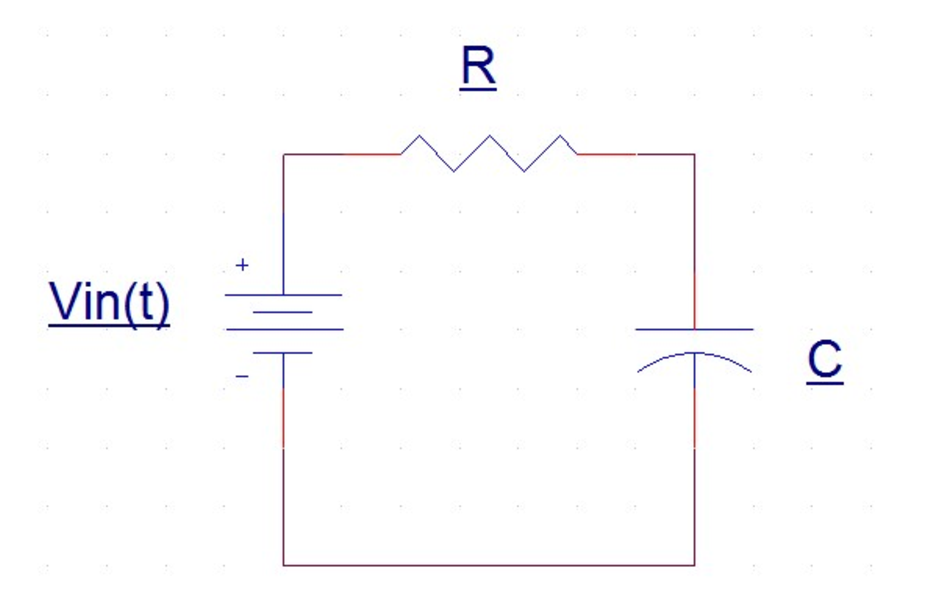
\includegraphics[width=0.50\textwidth]{RC.eps}
		\caption{Circuito RC}
		\label{fig:RC}
	\end{figure}

Como vemos, se trata de un circuito b\'asico RC, una fuente de voltaje en serie con una resistencia y un capacitor; y su funci\'on de transferencia esta dada de la siguiente manera.\medskip \\ Primero debemos encontrar su formula de balance de energ\'ias.
	\begin{center} $v_{in}(t) = v_{r}(t) + v_{c}(t)$\end{center}
Y esta tambi\'en se puede escribir como:
	\begin{center} $v_{in}(t) = R \cdot i_{c}(t) + v_{c}(t)$\end{center}
Pero sabemos que:
	\begin{center} $i_{c}(t) = \frac{d \cdot v_{c}(t)}{dt}$\end{center}
Y sustituyendo en la anterior.
	\begin{center} $v_{in}(t) = R\frac{dv_{c}(t)}{dt} + v_{c}(t)$\end{center}
Por ultimo aplicamos Laplace, y obtenemos lo siguiente:
	\begin{center} $V_{IN}(s) = RCsV_{c}(s) + V_{c}(s)$\end{center}
Y haciendo el despeje correspondiente para obtener una forma de la ecuaci\'on, con la cual podamos aplicar la anti-transformada de Laplace, obtenemos lo siguiente:
	\begin{equation}
		\centering
		H(s) = \frac{V_{c}(s)}{V_{IN}(s)} = \frac{\frac{1}{RC}}{s + \frac{1}{RC}}
		\label{ec:1}
	\end{equation}
Y ahora haremos lo mismo para un circuito RL.\medskip \\El circuito es el mismo que para RC pero con un inductor en vez de un capacitor. Este es mostrado en la Figura \ref{fig:RL}.\medskip

	\begin{figure}[h]
		\centering
			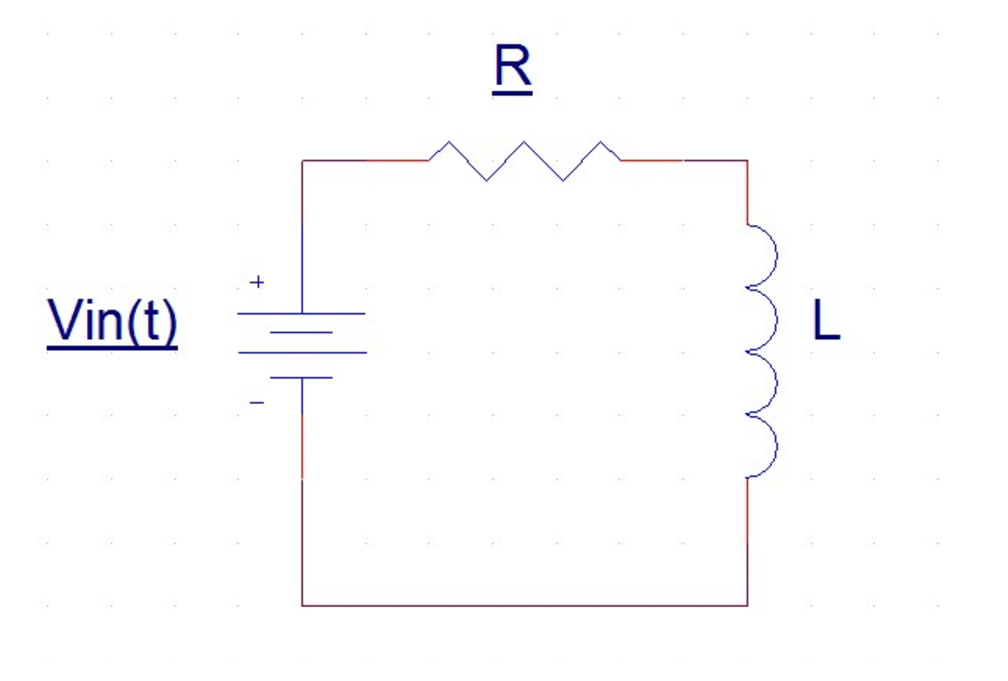
\includegraphics[width=0.50\textwidth]{RL.eps}
		\caption{Circuito RL}
		\label{fig:RL}
	\end{figure}

Y para obtener su funci\'on de transferencia las ecuaciones serian las siguientes:
	\begin{center} $v_{in}(t) = v_{R}(t) + v_{L}(t)$\end{center}
Y usando la igualdad de $v_{L}$ tenemos que:
	\begin{center} $v_{in}(t) = R \cdot i_{L}(t) + L \cdot \frac{di_{L}(t)}{dt}$\end{center}
Ahora aplicamos Laplace.
	\begin{center} $V_{IN}(s) = R \cdot I_{L}(s) + LSI_{L}(s)$\end{center}
Y finalmente obtenemos:
	\begin{equation}
		\centering
			H(s) = \frac {I_{L}(s)} {V_{IN}(s)} = \frac {\frac{1}{L}} {s + \frac{R}{L}}
		\label{ec:2}
	\end{equation}
Esta es la ecuaci\'on que nos interesa.\medskip \\ Conociendo la ecuaci\'on \ref{ec:1} y la ecuaci\'on \ref{ec:2}, entre otras que no pondremos en el reporte por simplicidad, podemos deducir que la forma est\'andar de una funci\'on de transferencia de primer orden tiene la forma:
	\begin{equation}
		\centering
			H(s) = \frac {bs + c} {s + a}
		\label{ec:3}
	\end{equation}
Y ahora que conocemos esta forma pasemos al siguiente paso.

	\section{Deduciendo la forma general para circuitos de primer orden}

Para esta secci\'on vamos a seguir justo donde nos quedamos, habiendo encontrado la forma est\'andar de $H(s)$ podemos encontrar el forma general para la salida de circuitos de primer orden; esta estar\'a dada por:
	\begin{center} $Y(s) = X(s) H(s)$ \end{center}
,donde:\medskip \\
	$H(s) =$ Funci\'on de transferencia\medskip \\
	$Y(s) =$ Salida del circuito\medskip \\
	$X(s) =$ Se\~nal escal\'on a la entrada del circuito\medskip \\
Ahora, como ya conocemos la forma estandar de $H(s)$, bastaria con encontrar la de $X(s)$, para nuestra suerte esto es bastante simple ya que al ser un escalon o $C$, su transformada de Laplace en cualquier caso sera directa, y sera de la forma:
	\begin{equation}
		\centering
			X(s) = \frac {1} {s}
		\label{ec:4}
	\end{equation}
Ahora podemos encontrar la forma est\'andar de $Y(s)$, y esta esta dada por:
	\begin{center} $Y(s) = \frac {1} {s} \cdot \frac {bs + c} {s + a}$ \end{center}
Aplicando fracciones parciales y un poco de \'algebra obtenemos:
	\begin{center} $Y(s) = \frac {c} {a} + (\frac {ab - c} {a}) e^{-at}$ \end{center}
Y finalmente regresando al dominio del tiempo obtenemos que:
	\begin{equation}
		\centering
			y(t) = \frac {c} {a} + (b - \frac {c} {a})e^{-at}
		\label{ec:5}
	\end{equation}

Y esta es la forma est\'andar de la salida de un circuito de primer orden; donde solo necesitamos encontrar los par\'ametros $a$, $b$ y $c$ para conocer la respuesta del circuito.

	\section{C\'odigo en SciLab} \label{sec:1}

Para esta seccion en base a la ecuaci\'on \ref{ec:5} crearemos un c\'odigo en SciLab que nos de, a partir de los par\'amentros $a$, $b$ y $c$ la forma de onda de la salida de cualquier circuito de primer orden. \medskip \\ Y el c\'odigo que generamos es el siguiente:

	\lstset{language=Scilab, breaklines=true, basicstyle=\footnotesize}
	\lstset{numbers=left, numberstyle=\tiny, stepnumber=1, numbersep=-30pt, frame=single}
	\begin{lstlisting} 
	function[y]=EcuGen(a,b,c)
	tau = 1/a;
	t = 0:tau/10:10*tau;
	n=length(t);
	u = c/a;
	if a~=0 then
		for i=1:n
		y(1,i) = u + ((b-u)*exp(-a*t(i)));
		end
	else
		for i=1:n
		y(n) = b;
		end
	end
	plot(t,y)
	endfunction
	\end{lstlisting}

Ahora explicaremos el c\'odigo a grandes rasgos; primero que nada, la funci\'on recibe los par\'ametros $a$,$b$ y $c$, y retorna un valor de $y$; ahora, despu\'es de analizar un poco la funci\'on, detectamos que $a$ es en realidad $\frac {1} {\tau}$, por lo cual, en la linea 2 del c\'odigo, despejando $a$, podemos obtener el valor de $\tau$; en la siguiente linea generamos un vector de 0 a $10\tau$, con divisiones que definir\'an la cantidad de valores que graficaremos en el eje X mas adelante, en este caso esta configurado para 100 valores, sin embargo, podr\'ia modificarse cambiando el denominador de los pasos o step que tendr\'a dicho vector\medskip \\Despu\'es en la linea 4 simplemente medimos el vector generado para conocer el numero de valores que graficaremos; la siguiente linea, la 5 genera una constante recurrente en la formula general de la salida, si revisamos la ecuaci\'on \ref{ec:5}, podemos ver que el termino $\frac {c} {a}$ se repite, y para simplificar el c\'odigo lo sustituiremos por $u$.\medskip \\A partir de aqu\'i, la linea 6, llegamos a la parte principal del c\'odigo; creamos un ciclo if que es por seguridad compara a con un 0, ya que si es igual se genera un error en el c\'odigo, porque en ese caso tendr\'iamos divisiones entre cero y eso es infinito, y eso acarrea problemas mas adelante. Sin embargo este error solo se dar\'ia si al calcular $a$, $b$ o $c$ el usuario se equivoca, ya que fuera de ese caso particular ning\'un sistema tiene en $a$ un valor de cero, porque eso significar\'ia que el sistema tiene $\tau = \infty$ y obviamente ning\'un sistema tiene ese valor para $\tau$; ahora, dentro de este ciclo tenemos otro ciclo for anidado, en el colocamos una variable con valor inicial 1, y que aumenta hasta llegar a el n\'umero de valores que tiene el vector de valores del eje X a evaluar, dentro de este ciclo se va creando otro vector que genera los valores de la salida para cada uno de los de entrada\medskip \\Y ya para terminar, en la pen\'ultima linea se genera una gr\'afica que contrapone los valores de 0 a $10\tau$(eje X), y los valores que se generan a la salida(eje Y), y se obtiene la respuesta de la salida del sistema evaluado.

	\section{Probando el c\'odigo}
	
Para terminar con esta primer parte de la practica probamos de manera r\'apida el c\'odigo generado. Lo haremos con un circuito RC de iguales caracter\'isticas al de la figura \ref{fig:RC}, asignaremos valores t\'ipicos; por ejemplo:\medskip \\ Para obtener un $\tau = 1ms$, conociendo que $\tau = RC$ y proponiendo un $C = 1 \mu F$, obtenemos un valor de $R = 1k\Omega$. \medskip \\ Conociendo estos valores y sabiendo que la formula general de este circuito en particular es la mostrada en la ecuaci\'on \ref{ec:1}, podemos encontrar los valores de $a$, $b$ y $c$ de la siguiente manera:
	\begin{center} $a = \frac {1} {RC} = \frac {1} {(1k\Omega)(1\mu F)} = 1000$ \end{center}
	\begin{center} $b = 0$ \end{center}
	\begin{center} $c = \frac {1} {RC} = \frac {1} {(1k\Omega)(1\mu F)} = 1000$ \end{center}
Y sustituyendo en el c\'odigo generado obtenemos la funci\'on de respuesta.

\begin{figure}[h]
	\centering
		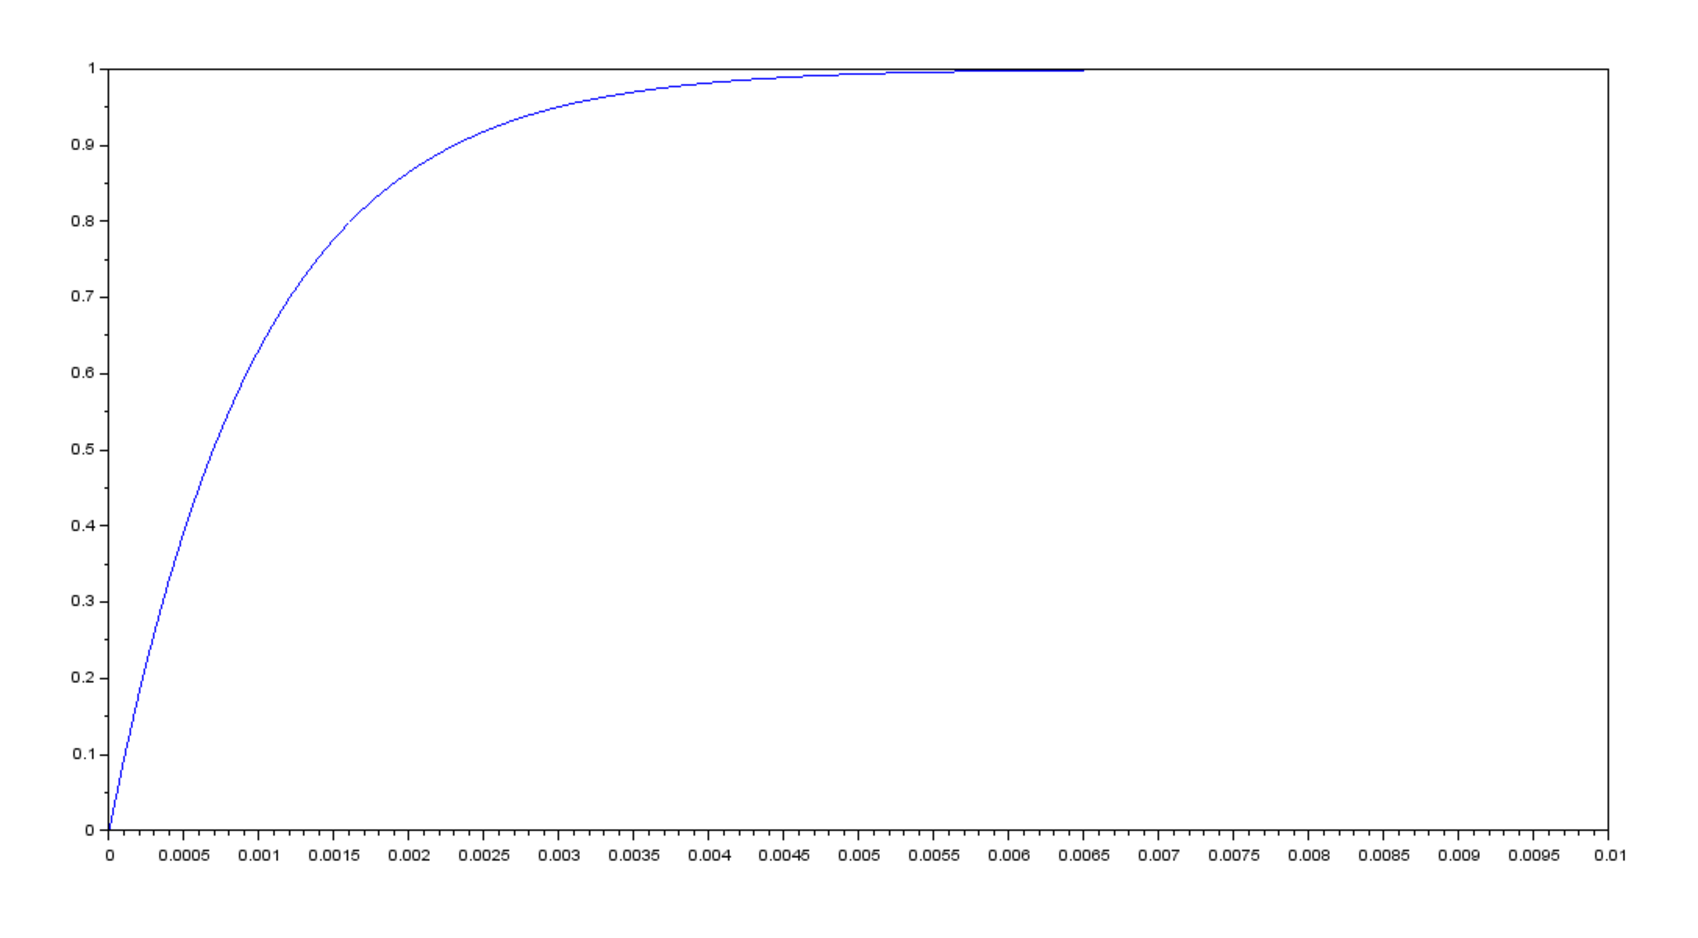
\includegraphics[width=1.00\textwidth]{Grafica1.eps}
	\caption{Respuesta a la salida del sistema propuesto.}
	\label{graf:1}
\end{figure}

 La respuesta de salida del sistema es mostrada en la figura \ref{graf:1}.

	\chapter{Ejercicio}

	\section{Ecuaci\'on de balance de energ\'ia}

Para esta parte del reporte trabajaremos con el sistema hidr\'aulico propuesto en la caratula de la practica.

\begin{figure}[h]
	\centering
		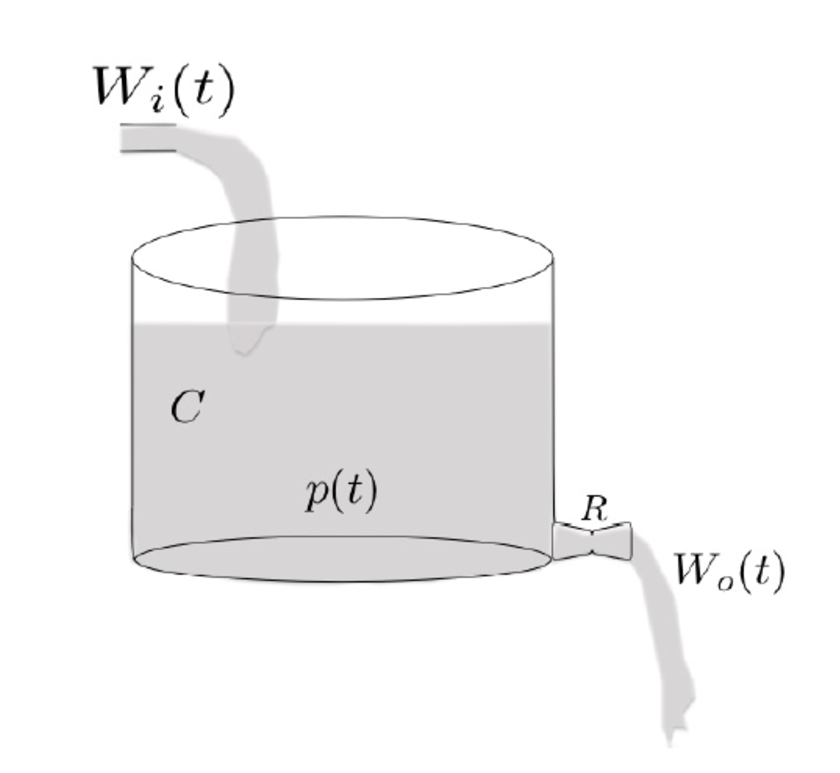
\includegraphics[width=0.50\textwidth]{tanque.eps}
	\caption{Sistema hidr\'aulico propuesto.}
	\label{fig:tanque}
\end{figure}

Para obtener la ecuaci\'on de balance de energ\'ia del sistema mostrado en la figura \ref{fig:tanque} necesitamos encontrar una ecuaci\'on con la siguiente estructura:
	\begin{center} $Energia_{generada} + Energia_{entrada} = Energia_{acumulada} + Energia_{salida}$ \end{center}
En el sistema notamos que no existe una energ\'ia generada, sin embargo si una energ\'ia de entrada, esta es el flujo de entrada del agua, llamada para el sistema $w_{i}(t)$, tambi\'en tenemos una energ\'ia acumulada, que es el agua en el tanque, esta se describe como $A \cdot \frac {h(t)} {dt} $, ya que depende tanto del area $A$ como de la altura $h$ sin embargo, como la altura es variable dependiendo de la entrada y salida del agua en un tiempo determinado, esta es dependiente del tiempo; y por ultimo tenemos la energ\'ia de salida, que es el flujo de agua a la salida, esta esta representada en el sistema como $w_{o}(t)$, y es proporcional a la resistencia R que oponga la boquilla de salida al flujo, ahora sabemos que este par\'ametro esta dado por $\frac {rgh} {R} $; por lo tanto sabemos que:

	\begin{equation}
		\centering
			w_{i}(t) = A \cdot \frac {dh(t)} {dt} + \frac {rgh(t)} {R}  
		\label{ec:6}
	\end{equation}

La ecuaci\'on \ref{ec:6} es la ecuaci\'on de balance de energ\'ia.

\section{Funci\'on de transferencia}

Para obtener la funci\'on de transferencia podemos hacer la analog\'ia del sistema anterior a un sistema el\'ectrico, observando un poco la forma de la funci\'on obtenida en la ecuaci\'on \ref{ec:6} notamos ciertas similitudes entre las variables hidr\'aulicas y las el\'ectricas, y haciendo la sustitucion de las mismas obtenemos una ecuacion de la siguiente forma:
Si $A = c$, $w_{i}(t) = i_{in}(t)$, $h(t) = v_{c}(t)$ y $\frac {R} {rg} = R$, entonces:
	\begin{equation}
		\centering
			i_(t) = c \cdot \frac {dv_{c}(t)} {dt} + \frac {v_{c}(t)} {(R} 
		\label{ec:7}
	\end{equation}
Utilizando esta ecuaci\'on podemos definir que:

\begin{figure}[h]
	\centering
		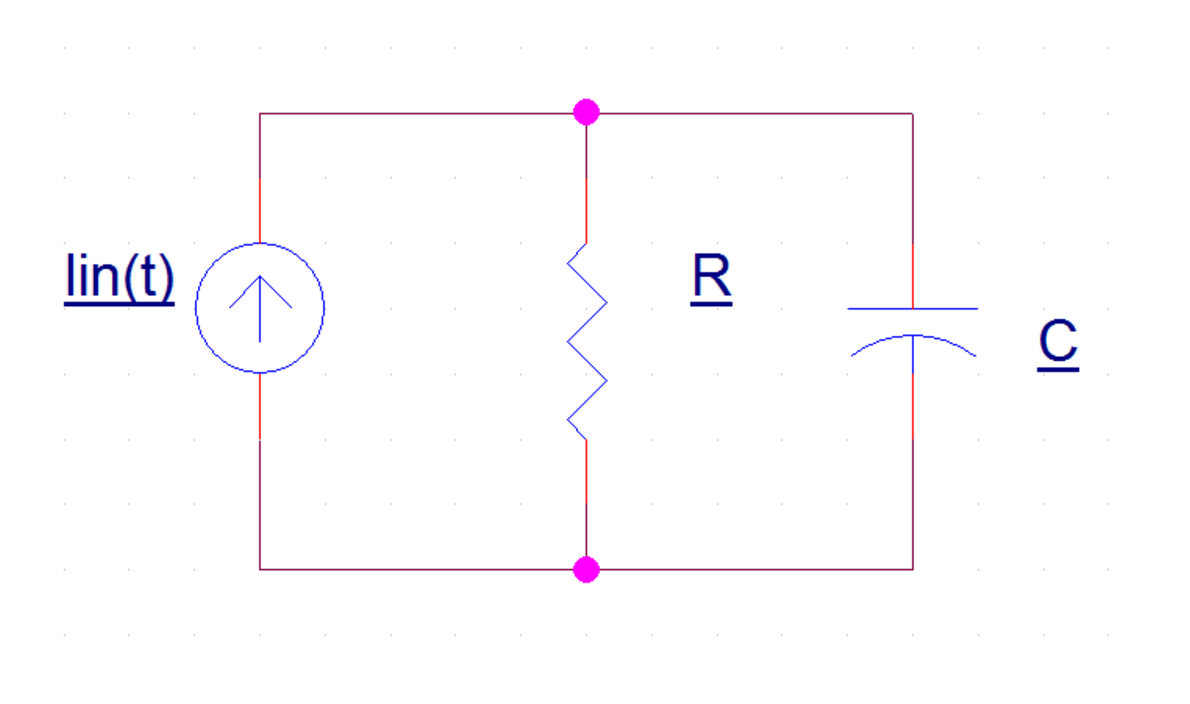
\includegraphics[width=0.50\textwidth]{RC2.eps}
	\caption{Circuito electrico equivalente al sistema hidraulico.}
	\label{fig:RC2}
\end{figure}

Aplicando transformada de Laplace a la ecuaci\'on \ref{ec:7} obtenemos:
	\begin{center}$I_(s) = C \cdot sV_{c}(s) + \frac {V_{c}(s)} {R)} $\end{center}
Y encontramos entonces que:
	\begin{equation}
		\centering
			\frac {V_{c}(s)} {I_{IN}(s)} = \frac {\frac {1} {C}} {s + (\frac {1} {RC})}
		\label{ec:8}
	\end{equation}
Entonces es la ecuaci\'on \ref{ec:8} la funci\'on de transferencia del sistema hidr\'aulico propuesto.

\section{C\'alculos con valores}

Bien, propongamos valores para el sistema, para no complicarnos entrando en detalles de sistemas hidr\'aulicos que son tardados, y hasta cierto punto innecesarios para el objetivo de la practica, nos aprovecharemos del hecho de que ya obtuvimos el equivalente el\'ectrico del sistema, por lo cual, propondremos variables hidr\'aulicas, y a partir de ellas encontraremos las variables el\'ectricas para el ejercicio, cuidando obviamente que sean congruentes con el tipo de sistema. \medskip \\Ahora que se aclaro ese punto vamos a iniciar; para empezar observemos la ecuaci\'on \ref{ec:8}, aqu\'i vemos que necesitamos valores para R y c, que ser\'an a su vez la resistencia de la salida del tanque y el \'area del mismo; para el \'area del tanque o C no hay problema, suponiendo que esta dada en metros podemos imaginar un tanque de muchas medidas, para nuestro caso en especifico lo estableceremos de 50cm o lo que es lo mismo 0.5m, as\'i que $C = 0.5$; despu\'es necesitamos R(el\'ectrica), esta esta dada por R(hidr\'aulica), r y g; donde r es el radio de la boquilla de salida del tanque, en nuestro caso sera de 5cm, o 0.05m, ademas necesitamos g, que es la gravedad, y todos sabemos que la gravedad es de $9.8m/s^{2}$ as\'i que esta parte no tiene ning\'un misterio; sin embargo para R, que es un par\'ametro dado por la construcci\'on del tanque no conocemos de que depende ni como funciona, as\'i que solo propongamos su valor en 1; y partiendo de esto sabemos que $R = \frac {R} {rg} = \frac {1} {(o.05)(9.8)} = 2.0408163$.\medskip \\ Ahora que conocemos esos valores pasemos a la siguiente secci\'on.
	
	\section{Graficando en SciLab}
	
Y a partir de los valores anteriores y la ecuaci\'on \ref{ec:8} podemos encontrar que:
	
	\begin{center}$a = \frac {R} {C} = 4.0816327$\end{center}
	\begin{center}$b = 0$\end{center}
	\begin{center}$c = \frac {1} {C} = 2$\end{center}
	
Y insertando esto en el c\'odigo generado en la secci\'on  \ref{sec:1} obtenemos la respuesta de la salida del tanque mostrada en la figura \ref{graf:2}.

\begin{figure}[h]
	\centering
		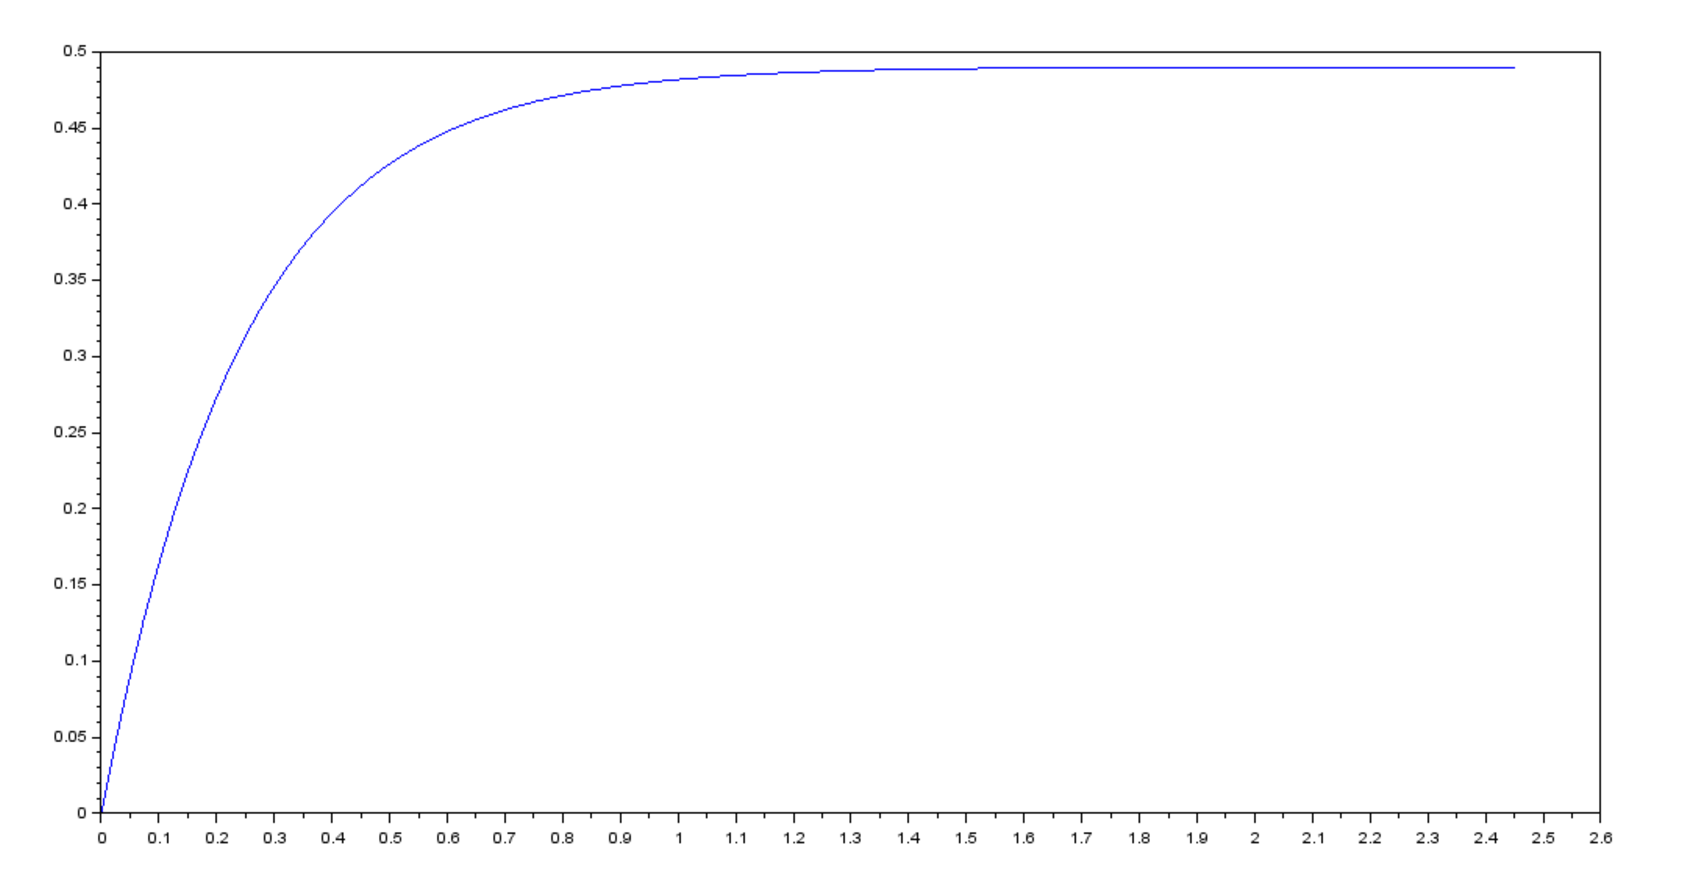
\includegraphics[width=1.00\textwidth]{Grafica2.eps}
	\caption{Respuesta de salida del sistema hidraulico propuesto.}
	\label{graf:2}
\end{figure}

Y analizando esta figura vemos que el tiempo de respuesta del sistema(eje X) para que el sistema sea estable, o al menos para que este por encima del 90 por ciento de su respuesta m\'axima es en aproximadamente 5s, y esto es muy conveniente ya que si buscamos $\tau$ por medio de la formula RC, tenemos que $\tau = RC = (2.04)(0.5) = 1.02$
por lo que $5\tau$ es en aproximadamente 5s.
La presente funci\'on de respuesta corresponde al lo que analogamente en un circuito el\'ectrico seria el proceso de carga de un capacitor, pero para el sistema hidr\'aulico representa la respuesta con respecto al tiempo de como se llena el tanque.

\chapter{Resultados y Conclusi\'ones}
\section{Resultados}
Durante la practica se obtuvo la capacidad para plantear el modelo matematico de un sistema de control de primer orden, as\'i como una funcion para scilab que permite obtener la respuesta en el tiempo de cualquier sistema de primer orden en base a los coeficientes de la ecuacion general de la funcion de transferencia. Gracias al codigo generado se pudo comprobar el comportamiento te\'orico de un sistema de primer orden, tambien pudo verse que el coeficiente $a$ siempre resulta ser el inverso de la constante de tiempo $\tau$. Todos los sistemas tienen a simple vista la misma forma para carga y descarga.   
\section{Discusi\'on} 
Para los sistemas de primer orden los resultados obtenidos pueden ser intuidos con facilidad ya que solo cuentan con un elemento que depende del tiempo, de tal modo que sin importar el tipo de sistema con el que se este trabajando el modelo matem\'atico en el dominio de la frecuencia es practicamente igual y se pueden hacer analog\'ias entre ellos.
\section{Conclusi\'ones}
Despues de todo el proceso llevado a cabo en esta pr\'actica, podemos ver la utilidad que tiene el conocer y comprender la metodolog\'ia para establecer el modelo matem\'tico de un sistema en base a las leyes f\'isicas que lo rigen, y aun mas importante saber establecer analogias entre sistemas para poder trasladarlos a su analogo el\'ectrico y as\'i desarrollarlos de manera simple, y poder saber si los resultados obtenidos son congruentes.  
%%%%%%%%%    R E F E R E N C I A S %%%%%%%%%%%%%
\chapter*{Referencias}
[1] Classic Control Theory 101 Laboratory session 1. Gerardo Marx Ch\'avez Campos
web site: sagitario.itmorelia.edu.mx/gmarx/, descargado Oct. 25 de 2017.\medskip\\
$\rm{[2]}$ Dinamica y Control de procesos. Funci\'on de transferencia.
web site: www.grupovirtus.org, descargado Oct. 26 de 2017.
\end{document}
%Las referencias se agregan con \cite{keyCite}



